\documentclass{standalone}
\usepackage{tikz}
\usetikzlibrary{patterns, positioning}


\begin{document}
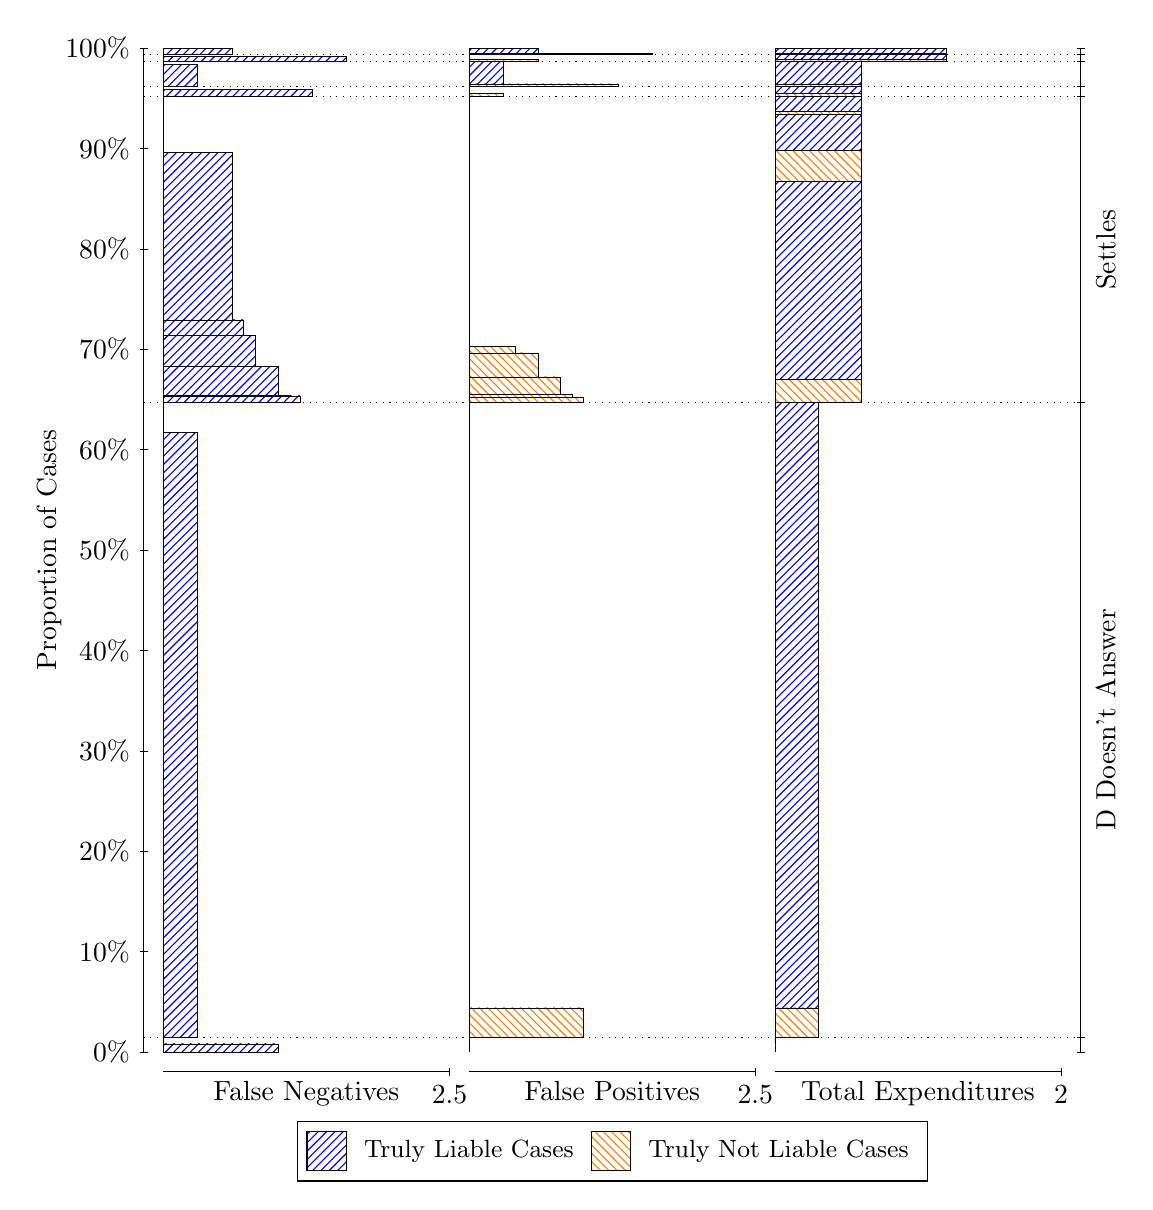
\begin{tikzpicture}
\draw[black, very thin] (1.5,1.75) -- (1.5,14.5);
\node[rotate=90, text=black, anchor=center] at (0.3, 8.125) {Proportion of Cases};
\draw[black, very thin] (1.45,1.75) -- (1.55,1.75);
\node[text=black, anchor=east] at (1.45, 1.75) {0\%};
\draw[black, very thin] (1.45,3.025) -- (1.55,3.025);
\node[text=black, anchor=east] at (1.45, 3.025) {10\%};
\draw[black, very thin] (1.45,4.3) -- (1.55,4.3);
\node[text=black, anchor=east] at (1.45, 4.3) {20\%};
\draw[black, very thin] (1.45,5.575) -- (1.55,5.575);
\node[text=black, anchor=east] at (1.45, 5.575) {30\%};
\draw[black, very thin] (1.45,6.85) -- (1.55,6.85);
\node[text=black, anchor=east] at (1.45, 6.85) {40\%};
\draw[black, very thin] (1.45,8.125) -- (1.55,8.125);
\node[text=black, anchor=east] at (1.45, 8.125) {50\%};
\draw[black, very thin] (1.45,9.4) -- (1.55,9.4);
\node[text=black, anchor=east] at (1.45, 9.4) {60\%};
\draw[black, very thin] (1.45,10.675) -- (1.55,10.675);
\node[text=black, anchor=east] at (1.45, 10.675) {70\%};
\draw[black, very thin] (1.45,11.95) -- (1.55,11.95);
\node[text=black, anchor=east] at (1.45, 11.95) {80\%};
\draw[black, very thin] (1.45,13.225) -- (1.55,13.225);
\node[text=black, anchor=east] at (1.45, 13.225) {90\%};
\draw[black, very thin] (1.45,14.5) -- (1.55,14.5);
\node[text=black, anchor=east] at (1.45, 14.5) {100\%};

\draw[black, very thin] (13.4,1.75) -- (13.4,14.5);
\draw[black, very thin] (13.35,1.75) -- (13.45,1.75);
\node[anchor=west] at (13.35, 1.75) {};
\draw[black, very thin] (13.35,1.9362) -- (13.45,1.9362);
\node[anchor=west] at (13.35, 1.9362) {};
\draw[black, very thin] (13.35,9.9968) -- (13.45,9.9968);
\node[anchor=west] at (13.35, 9.9968) {};
\draw[black, very thin] (13.35,13.886) -- (13.45,13.886);
\node[anchor=west] at (13.35, 13.886) {};
\draw[black, very thin] (13.35,14.008) -- (13.45,14.008);
\node[anchor=west] at (13.35, 14.008) {};
\draw[black, very thin] (13.35,14.331) -- (13.45,14.331);
\node[anchor=west] at (13.35, 14.331) {};
\draw[black, very thin] (13.35,14.421) -- (13.45,14.421);
\node[anchor=west] at (13.35, 14.421) {};
\draw[black, very thin] (13.35,14.5) -- (13.45,14.5);
\node[anchor=west] at (13.35, 14.5) {};

\draw[black, very thin, pattern color=blue, pattern=north east lines] (1.75,1.75) rectangle (3.2033,1.8527);
\draw[black, very thin, pattern color=orange, pattern=north west lines] (1.75,1.8527) rectangle (1.75,1.9362);
\draw[black, very thin, pattern color=blue, pattern=north east lines] (1.75,1.9362) rectangle (2.186,9.6231);
\draw[black, very thin, pattern color=orange, pattern=north west lines] (1.75,9.6231) rectangle (1.75,9.9968);
\draw[black, very thin, pattern color=blue, pattern=north east lines] (1.75,9.9968) rectangle (3.494,10.082);
\draw[black, very thin, pattern color=blue, pattern=north east lines] (1.75,10.082) rectangle (3.3487,10.087);
\draw[black, very thin, pattern color=blue, pattern=north east lines] (1.75,10.087) rectangle (3.2033,10.457);
\draw[black, very thin, pattern color=blue, pattern=north east lines] (1.75,10.457) rectangle (2.9127,10.85);
\draw[black, very thin, pattern color=blue, pattern=north east lines] (1.75,10.85) rectangle (2.7673,11.046);
\draw[black, very thin, pattern color=blue, pattern=north east lines] (1.75,11.046) rectangle (2.622,13.174);
\draw[black, very thin, pattern color=orange, pattern=north west lines] (1.75,13.174) rectangle (1.75,13.886);
\draw[black, very thin, pattern color=blue, pattern=north east lines] (1.75,13.886) rectangle (3.6393,13.972);
\draw[black, very thin, pattern color=orange, pattern=north west lines] (1.75,13.972) rectangle (1.75,14.008);
\draw[black, very thin, pattern color=blue, pattern=north east lines] (1.75,14.008) rectangle (2.186,14.295);
\draw[black, very thin, pattern color=orange, pattern=north west lines] (1.75,14.295) rectangle (1.75,14.331);
\draw[black, very thin, pattern color=blue, pattern=north east lines] (1.75,14.331) rectangle (4.0753,14.396);
\draw[black, very thin, pattern color=orange, pattern=north west lines] (1.75,14.396) rectangle (1.75,14.421);
\draw[black, very thin, pattern color=blue, pattern=north east lines] (1.75,14.421) rectangle (2.622,14.493);
\draw[black, very thin, pattern color=orange, pattern=north west lines] (1.75,14.493) rectangle (1.75,14.5);
\draw[black, very thin, pattern color=orange, pattern=north west lines] (5.6333,1.75) rectangle (5.6333,1.8336);
\draw[black, very thin, pattern color=blue, pattern=north east lines] (5.6333,1.8336) rectangle (5.6333,1.9362);
\draw[black, very thin, pattern color=orange, pattern=north west lines] (5.6333,1.9362) rectangle (7.0867,2.3099);
\draw[black, very thin, pattern color=blue, pattern=north east lines] (5.6333,2.3099) rectangle (5.6333,9.9968);
\draw[black, very thin, pattern color=orange, pattern=north west lines] (5.6333,9.9968) rectangle (7.0867,10.067);
\draw[black, very thin, pattern color=orange, pattern=north west lines] (5.6333,10.067) rectangle (6.9413,10.101);
\draw[black, very thin, pattern color=orange, pattern=north west lines] (5.6333,10.101) rectangle (6.796,10.324);
\draw[black, very thin, pattern color=orange, pattern=north west lines] (5.6333,10.324) rectangle (6.5053,10.626);
\draw[black, very thin, pattern color=orange, pattern=north west lines] (5.6333,10.626) rectangle (6.36,10.629);
\draw[black, very thin, pattern color=orange, pattern=north west lines] (5.6333,10.629) rectangle (6.2147,10.709);
\draw[black, very thin, pattern color=blue, pattern=north east lines] (5.6333,10.709) rectangle (5.6333,13.886);
\draw[black, very thin, pattern color=orange, pattern=north west lines] (5.6333,13.886) rectangle (6.0693,13.923);
\draw[black, very thin, pattern color=blue, pattern=north east lines] (5.6333,13.923) rectangle (5.6333,14.008);
\draw[black, very thin, pattern color=orange, pattern=north west lines] (5.6333,14.008) rectangle (7.5227,14.045);
\draw[black, very thin, pattern color=blue, pattern=north east lines] (5.6333,14.045) rectangle (6.0693,14.331);
\draw[black, very thin, pattern color=orange, pattern=north west lines] (5.6333,14.331) rectangle (6.5053,14.357);
\draw[black, very thin, pattern color=blue, pattern=north east lines] (5.6333,14.357) rectangle (5.6333,14.421);
\draw[black, very thin, pattern color=orange, pattern=north west lines] (5.6333,14.421) rectangle (7.9587,14.429);
\draw[black, very thin, pattern color=blue, pattern=north east lines] (5.6333,14.429) rectangle (6.5053,14.5);
\draw[black, very thin, pattern color=orange, pattern=north west lines] (9.5167,1.75) rectangle (9.5167,1.8336);
\draw[black, very thin, pattern color=blue, pattern=north east lines] (9.5167,1.8336) rectangle (9.5167,1.9362);
\draw[black, very thin, pattern color=orange, pattern=north west lines] (9.5167,1.9362) rectangle (10.062,2.3099);
\draw[black, very thin, pattern color=blue, pattern=north east lines] (9.5167,2.3099) rectangle (10.062,9.9968);
\draw[black, very thin, pattern color=orange, pattern=north west lines] (9.5167,9.9968) rectangle (10.607,10.289);
\draw[black, very thin, pattern color=blue, pattern=north east lines] (9.5167,10.289) rectangle (10.607,12.811);
\draw[black, very thin, pattern color=orange, pattern=north west lines] (9.5167,12.811) rectangle (10.607,13.196);
\draw[black, very thin, pattern color=blue, pattern=north east lines] (9.5167,13.196) rectangle (10.607,13.656);
\draw[black, very thin, pattern color=orange, pattern=north west lines] (9.5167,13.656) rectangle (10.607,13.691);
\draw[black, very thin, pattern color=blue, pattern=north east lines] (9.5167,13.691) rectangle (10.607,13.886);
\draw[black, very thin, pattern color=orange, pattern=north west lines] (9.5167,13.886) rectangle (10.607,13.923);
\draw[black, very thin, pattern color=blue, pattern=north east lines] (9.5167,13.923) rectangle (10.607,14.008);
\draw[black, very thin, pattern color=orange, pattern=north west lines] (9.5167,14.008) rectangle (10.607,14.045);
\draw[black, very thin, pattern color=blue, pattern=north east lines] (9.5167,14.045) rectangle (10.607,14.331);
\draw[black, very thin, pattern color=orange, pattern=north west lines] (9.5167,14.331) rectangle (11.697,14.357);
\draw[black, very thin, pattern color=blue, pattern=north east lines] (9.5167,14.357) rectangle (11.697,14.421);
\draw[black, very thin, pattern color=orange, pattern=north west lines] (9.5167,14.421) rectangle (11.697,14.429);
\draw[black, very thin, pattern color=blue, pattern=north east lines] (9.5167,14.429) rectangle (11.697,14.5);
\draw[black, dotted] (1.5,1.9362) -- (13.4,1.9362);
\draw[black, dotted] (1.5,9.9968) -- (13.4,9.9968);
\draw[black, dotted] (1.5,13.886) -- (13.4,13.886);
\draw[black, dotted] (1.5,14.008) -- (13.4,14.008);
\draw[black, dotted] (1.5,14.331) -- (13.4,14.331);
\draw[black, dotted] (1.5,14.421) -- (13.4,14.421);
\draw[black, very thin] (1.75,1.5) -- (5.3833,1.5);
\node[text=black, anchor=north] at (3.5667, 1.5) {False Negatives};
\draw[black, very thin] (5.3833,1.45) -- (5.3833,1.55);
\node[text=black, anchor=north] at (5.3833, 1.45) {2.5};

\draw[black, very thin] (5.6333,1.5) -- (9.2667,1.5);
\node[text=black, anchor=north] at (7.45, 1.5) {False Positives};
\draw[black, very thin] (9.2667,1.45) -- (9.2667,1.55);
\node[text=black, anchor=north] at (9.2667, 1.45) {2.5};

\draw[black, very thin] (9.5167,1.5) -- (13.15,1.5);
\node[text=black, anchor=north] at (11.333, 1.5) {Total Expenditures};
\draw[black, very thin] (13.15,1.45) -- (13.15,1.55);
\node[text=black, anchor=north] at (13.15, 1.45) {2};


\node[text=black, centered, rotate=90] at (13.72, 5.9665) {D Doesn't Answer};
\node[text=black, centered, rotate=90] at (13.72, 11.942) {Settles};





\draw (7.449999999999999,1.5) node[draw=none] (baseCoordinate) {};
\begin{scope}[align=center]
        \matrix[scale=0.5, draw=black, below=0.5cm of baseCoordinate, nodes={draw}, column sep=0.1cm]{
            \node[rectangle, draw, minimum width=0.5cm, minimum height=0.5cm, pattern color=blue, pattern=north east lines] {}; &
            \node[draw=none, font=\small, text=black] (B) {Truly Liable Cases}; &
            \node[rectangle, draw, minimum width=0.5cm, minimum height=0.5cm, pattern color=orange, pattern=north west lines] {}; &
            \node[draw=none, font=\small, text=black] (B) {Truly Not Liable Cases}; \\
            };
\end{scope}

\end{tikzpicture}
\end{document}